\section{Discussion of Results}
\label{sec:discussionofresults}

\subsection{Influence of some parameters in our model}

\subsubsection{Influence of \texttt{maxAgentupdate}}
\label{sec:maxAgentUpdate}
As figure \ref{influencemaxAgentUpdate} shows the value for
\texttt{maxAgentupdate} just gives us a different scaling of the time axis. If
it is bigger the total residual rises faster while if it is smaller the total
residual rises slower. As a result of this a change in the value of
\texttt{maxAgentupdate} could help to speed up the simulation in order to get
quicker results.

\begin{figure}
\centering
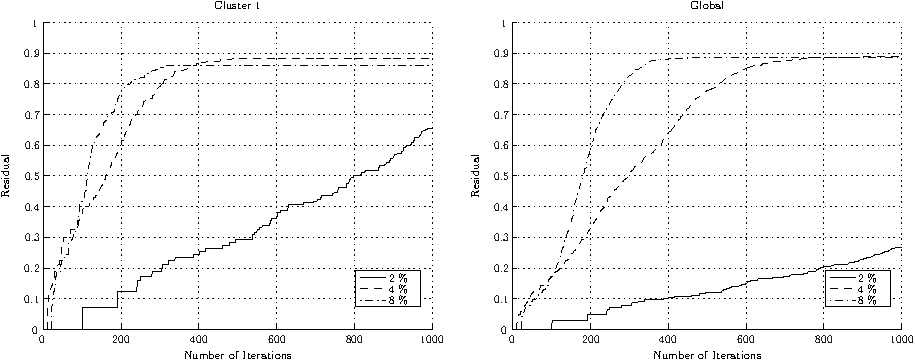
\includegraphics[width= \textwidth]{influenceOfmaxUpdate/influenceMaxAgentUpdate.pdf}
\caption{On the left the residual for the cluster in which the riots started is
  plotted while on the right the global residual, \ie, all three cluster
  combined, is shown. In both it is shown for values of 0.02, 0.04 and 0.08 of
  \texttt{maxAgentupdate}}
\label{influencemaxAgentUpdate}
\end{figure}


\subsubsection{Influence of \texttt{noize}}
\label{sec:influencenoize}
As figure \ref{influencenoize} shows, the noize could have quite an influence on the results of the simulation. In our network we have in total 1200 nodes. All the simulations in figure \ref{influencenoize} have the same \texttt{maxUpdate}=0.02. This means that in every time step 24 agents get updated. If the noize is now for example 0.01 only 0.24 agents choose randomly their state. In the case of a noize of 0.1 get 2.4 agents every time step a randomly after a uniform distribution chosen mind state. After this "noize update" the concerned agents are removed from the sequential update list so that they could not be updated twice.\\
As figure \ref{influencenoize} now shows and explained above a noize of 0.01 does not really change the results of the simulation as it has nearly no influence. But as the series of five plots on the right in figure \ref{influencenoize} shows a noize of 10 $\%$ does have quite a big influence on the results of the simulation. Before this big noize the riots where not really starting in the networks now they spread quickly.\\
Compared to reality we think that the noize tends to be close to 0. Who is just completly random changing his mind? It could be that some people change their mind independently from their neighbors and these should be covered by the noize. We think that a noize in reality should be something between 0 and 0.06.

\begin{figure}
\centering
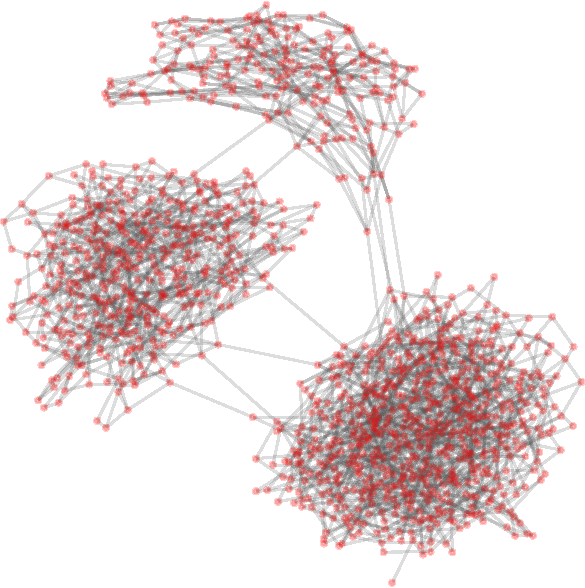
\includegraphics[width=0.25\textwidth]{batchRun__kHalf=2-2-2_maxUpdate=0.02_noize=0_nbrDepth=1/network0-crop.pdf}
\hfill
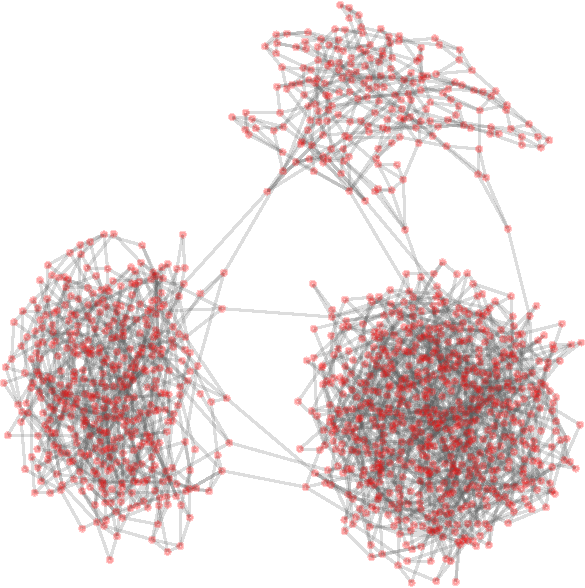
\includegraphics[width=0.25\textwidth]{batchRun__kHalf=2-2-2_maxUpdate=0.02_noize=0.01_nbrDepth=1/network0-crop.pdf}
\hfill
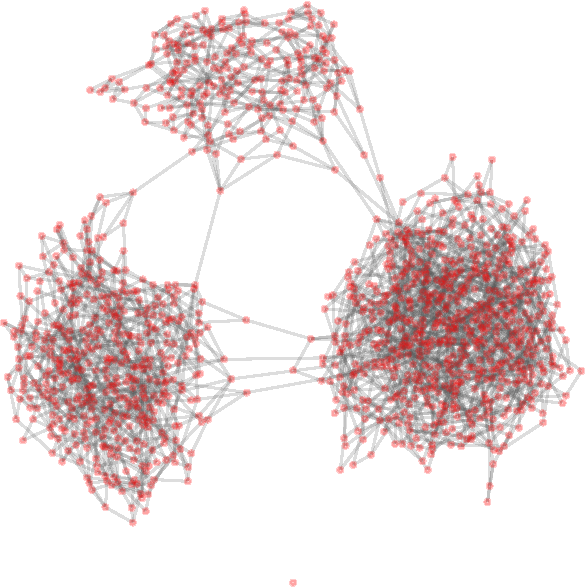
\includegraphics[width=0.25\textwidth]{batchRun__kHalf=2-2-2_maxUpdate=0.02_noize=0.1_nbrDepth=1/network0-crop.pdf}

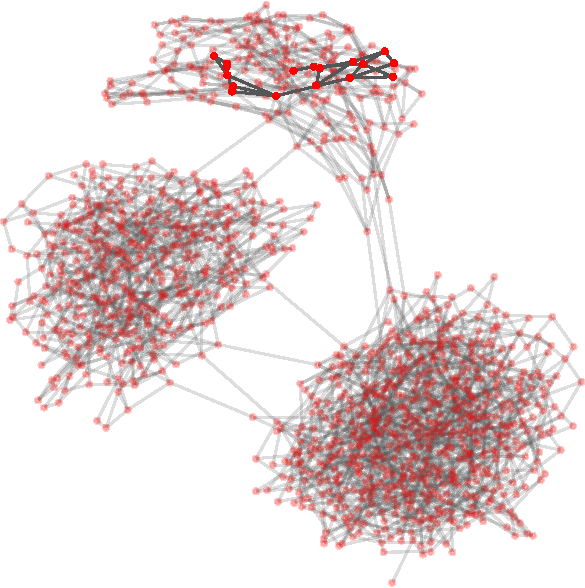
\includegraphics[width=0.25\textwidth]{batchRun__kHalf=2-2-2_maxUpdate=0.02_noize=0_nbrDepth=1/network250-crop.pdf}
\hfill
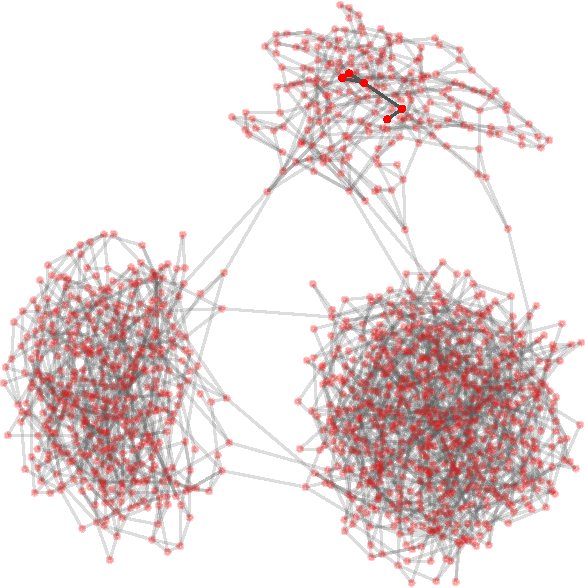
\includegraphics[width=0.25\textwidth]{batchRun__kHalf=2-2-2_maxUpdate=0.02_noize=0.01_nbrDepth=1/network250-crop.pdf}
\hfill
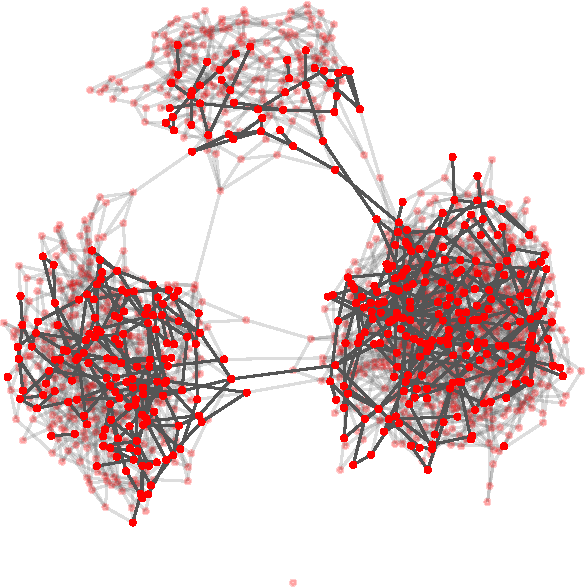
\includegraphics[width=0.25\textwidth]{batchRun__kHalf=2-2-2_maxUpdate=0.02_noize=0.1_nbrDepth=1/network250-crop.pdf}

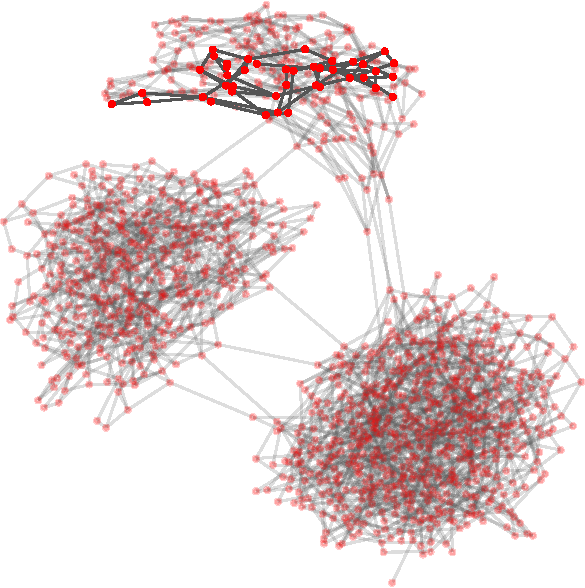
\includegraphics[width=0.25\textwidth]{batchRun__kHalf=2-2-2_maxUpdate=0.02_noize=0_nbrDepth=1/network500-crop.pdf}
\hfill
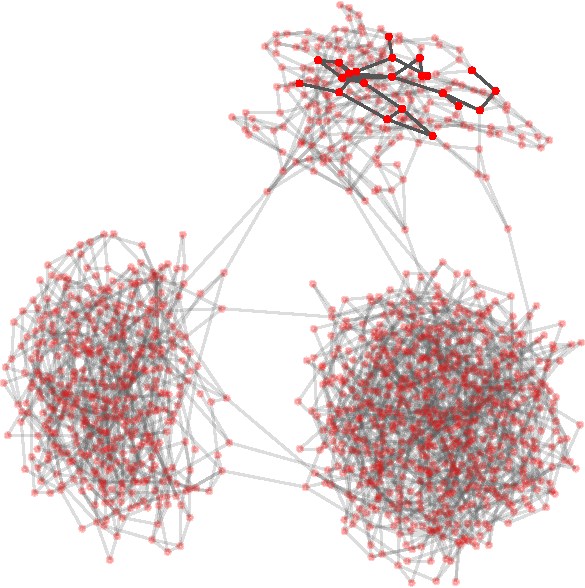
\includegraphics[width=0.25\textwidth]{batchRun__kHalf=2-2-2_maxUpdate=0.02_noize=0.01_nbrDepth=1/network500-crop.pdf}
\hfill
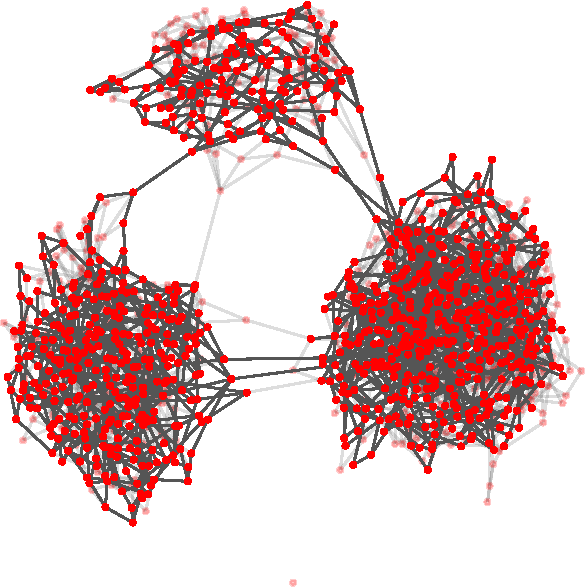
\includegraphics[width=0.25\textwidth]{batchRun__kHalf=2-2-2_maxUpdate=0.02_noize=0.1_nbrDepth=1/network500-crop.pdf}


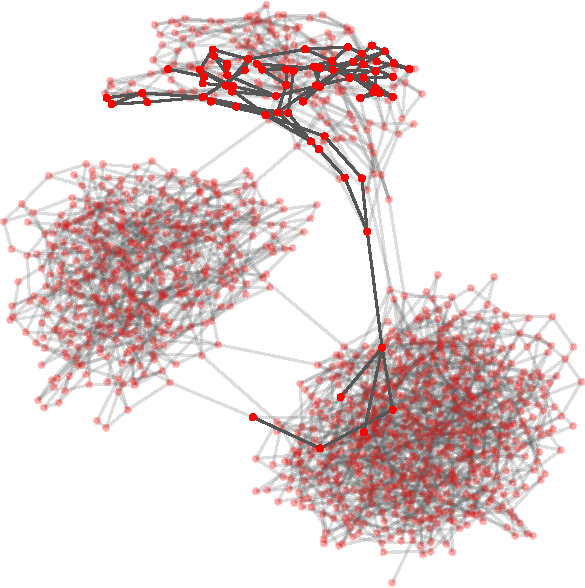
\includegraphics[width=0.25\textwidth]{batchRun__kHalf=2-2-2_maxUpdate=0.02_noize=0_nbrDepth=1/network750-crop.pdf}
\hfill
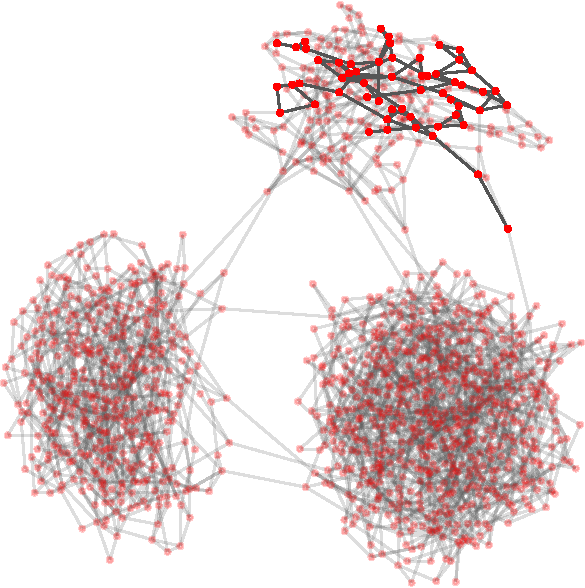
\includegraphics[width=0.25\textwidth]{batchRun__kHalf=2-2-2_maxUpdate=0.02_noize=0.01_nbrDepth=1/network750-crop.pdf}
\hfill
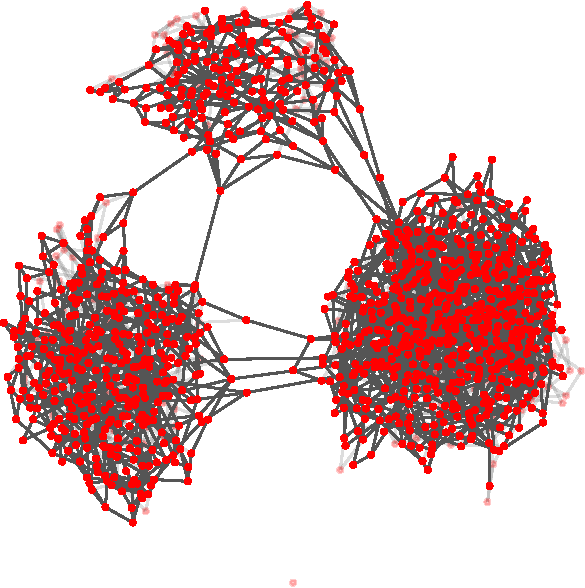
\includegraphics[width=0.25\textwidth]{batchRun__kHalf=2-2-2_maxUpdate=0.02_noize=0.1_nbrDepth=1/network750-crop.pdf}

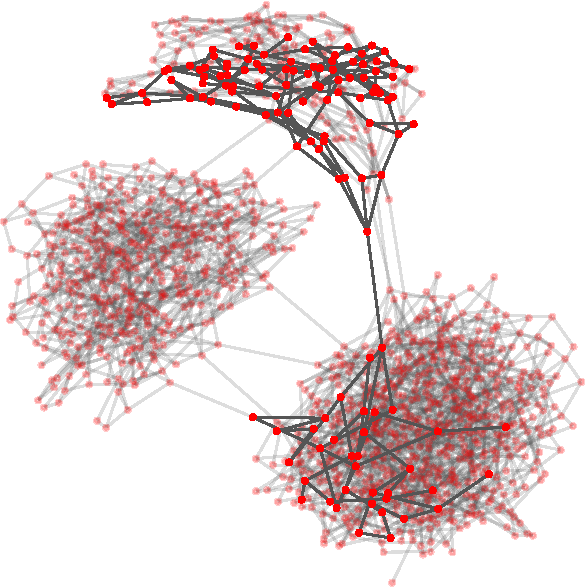
\includegraphics[width=0.25\textwidth]{batchRun__kHalf=2-2-2_maxUpdate=0.02_noize=0_nbrDepth=1/network1000-crop.pdf}
\hfill
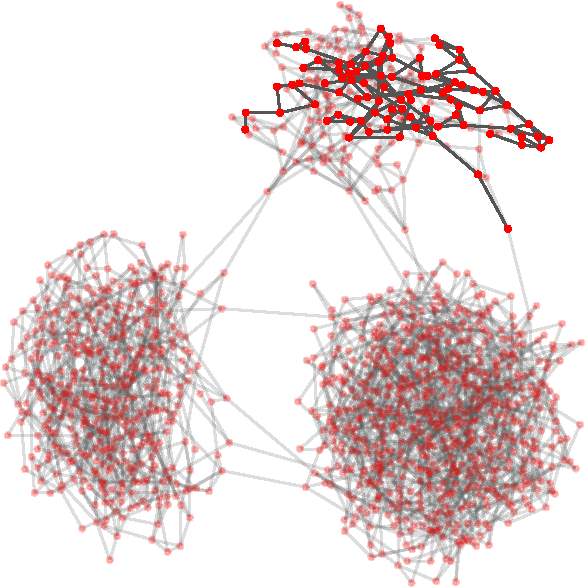
\includegraphics[width=0.25\textwidth]{batchRun__kHalf=2-2-2_maxUpdate=0.02_noize=0.01_nbrDepth=1/network1000-crop.pdf}
\hfill
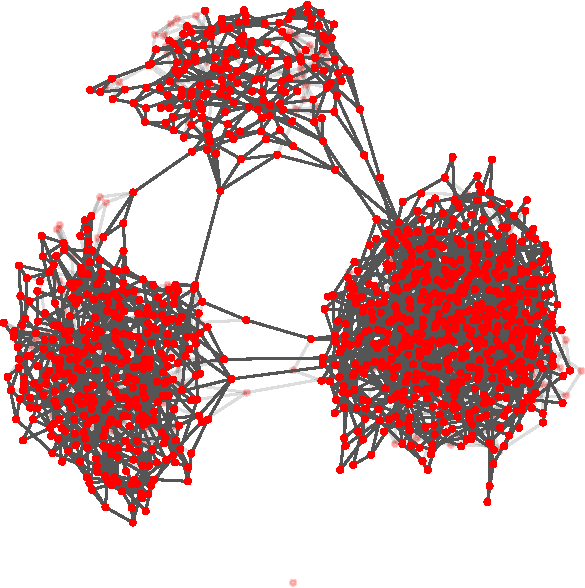
\includegraphics[width=0.25\textwidth]{batchRun__kHalf=2-2-2_maxUpdate=0.02_noize=0.1_nbrDepth=1/network1000-crop.pdf}

\caption{The influence of the noize for the three cases with on the left noize = 0, in the middle 0.01 and on the right 0.1. From top to bottom are the different time steps with the beginning and then increasing in 250 time steps till a 100 time steps.}
\label{influencenoize}
\end{figure}



\subsubsection{Influence of \texttt{nbrDepth} = Neighbor Depth}
\label{sec:nbrDepth}

\begin{figure}
\centering
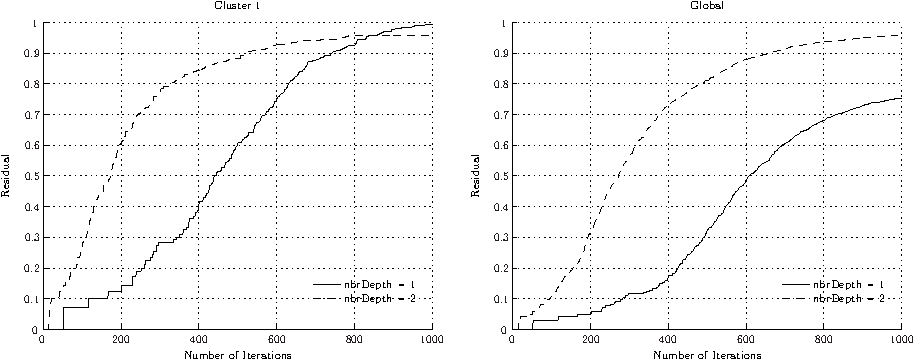
\includegraphics[width= \textwidth]{influenceOfNbrDepth/influenceNbrDepth.pdf}
\caption{The residuals for neighbor depth 1 (on the left) and 2 (on the right) compared for a small world network and a randrom graph. The other parameters for the small world network are as in \ref{influencenbrdepth} and for the random graph as in \ref{influenceNBRdepthRANDOM}.}
\label{residualNBRdepth}
\end{figure}

As figure \ref{influencenbrdepth} shows has an iteration over neighbor depth 2 a faster dynamic compared to a neighbor depth of 1. Through a neighbor depth of 2 there is also a quicker jump over from one cluster to the next cluster. This could be explained simply because there is a high probability that with one node in between there is a link between two clusters. The to this plot belonging residuals are shown in figure \ref{residualNBRdepth}.

\begin{figure}
\centering
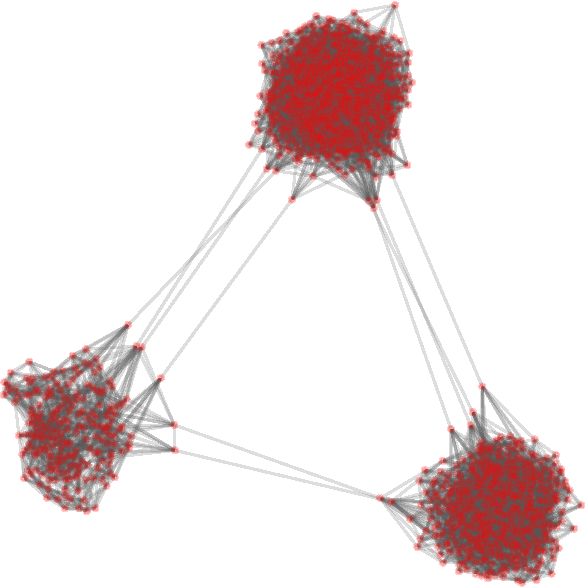
\includegraphics[width=0.3\textwidth]{batchRun__kHalf=6-6-6_maxUpdate=0.02_noize=0_nbrDepth=1/network0-crop.pdf}
\hskip2cm
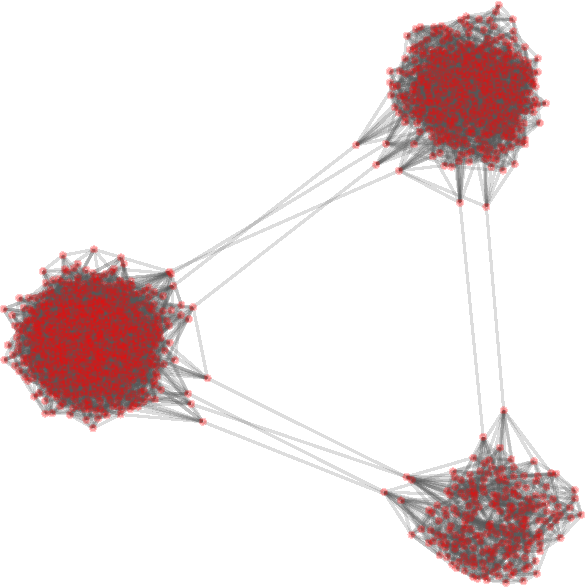
\includegraphics[width=0.3\textwidth]{batchRun__kHalf=6-6-6_maxUpdate=0.02_noize=0_nbrDepth=2/network0-crop.pdf}

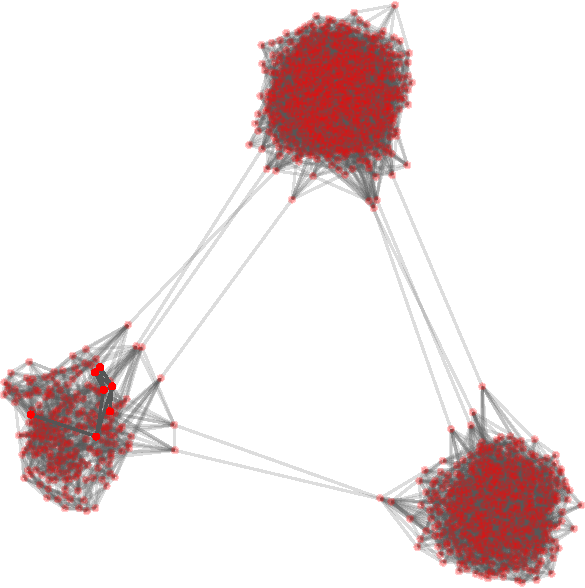
\includegraphics[width=0.3\textwidth]{batchRun__kHalf=6-6-6_maxUpdate=0.02_noize=0_nbrDepth=1/network250-crop.pdf}
\hskip2cm
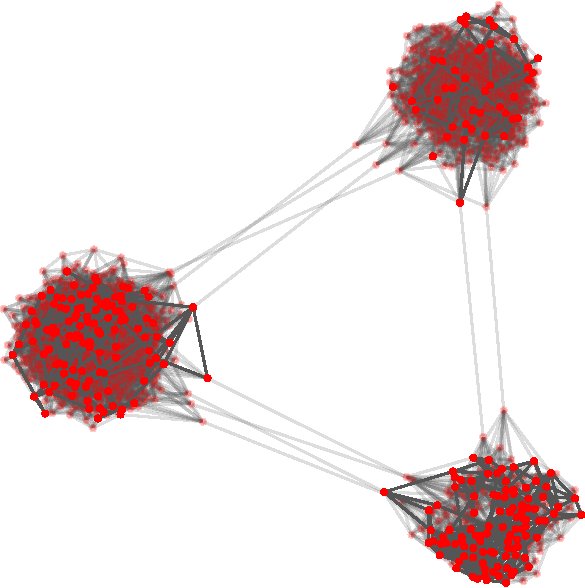
\includegraphics[width=0.3\textwidth]{batchRun__kHalf=6-6-6_maxUpdate=0.02_noize=0_nbrDepth=2/network250-crop.pdf}

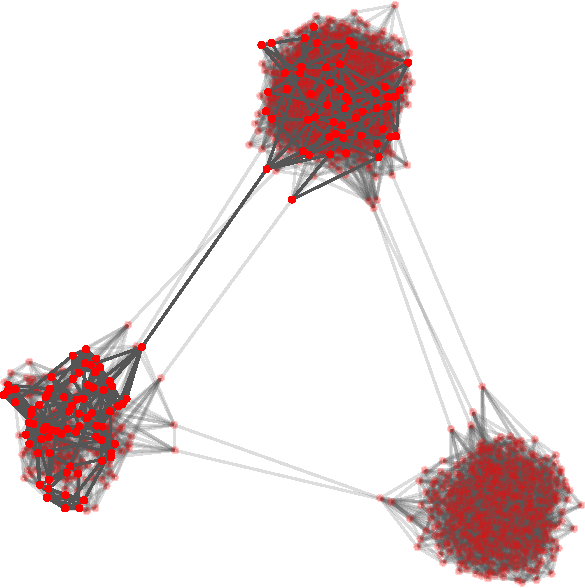
\includegraphics[width=0.3\textwidth]{batchRun__kHalf=6-6-6_maxUpdate=0.02_noize=0_nbrDepth=1/network500-crop.pdf}
\hskip2cm
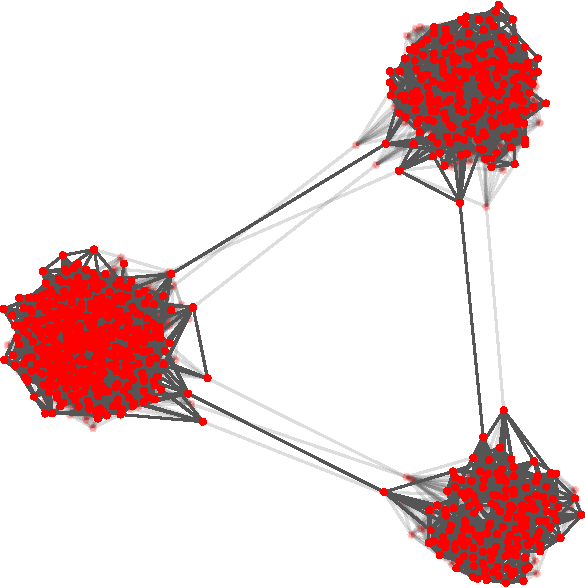
\includegraphics[width=0.3\textwidth]{batchRun__kHalf=6-6-6_maxUpdate=0.02_noize=0_nbrDepth=2/network500-crop.pdf}

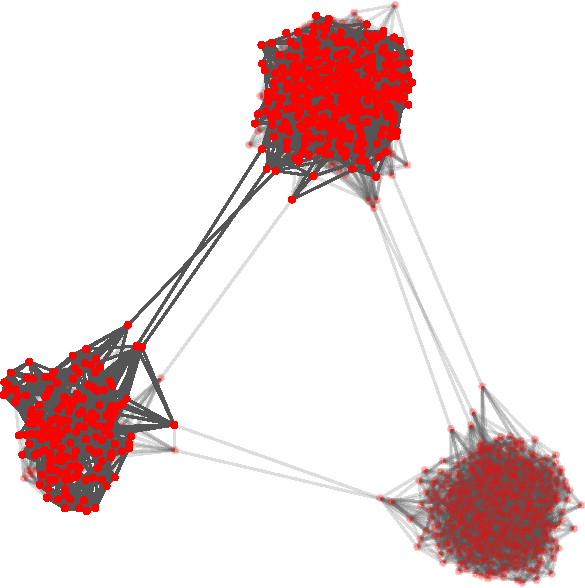
\includegraphics[width=0.3\textwidth]{batchRun__kHalf=6-6-6_maxUpdate=0.02_noize=0_nbrDepth=1/network750-crop.pdf}
\hskip2cm
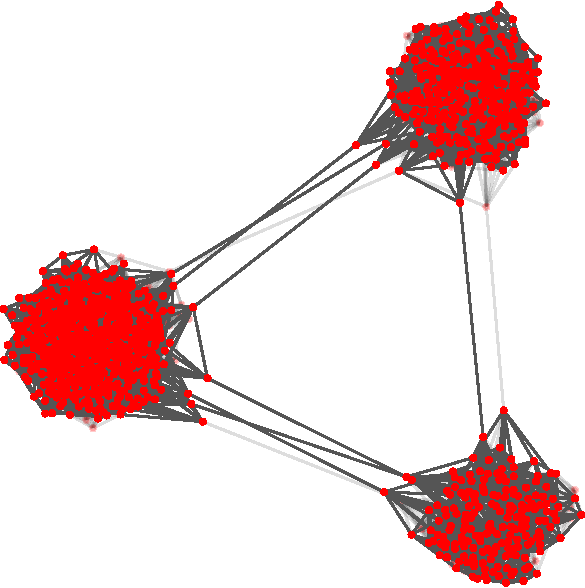
\includegraphics[width=0.3\textwidth]{batchRun__kHalf=6-6-6_maxUpdate=0.02_noize=0_nbrDepth=2/network750-crop.pdf}

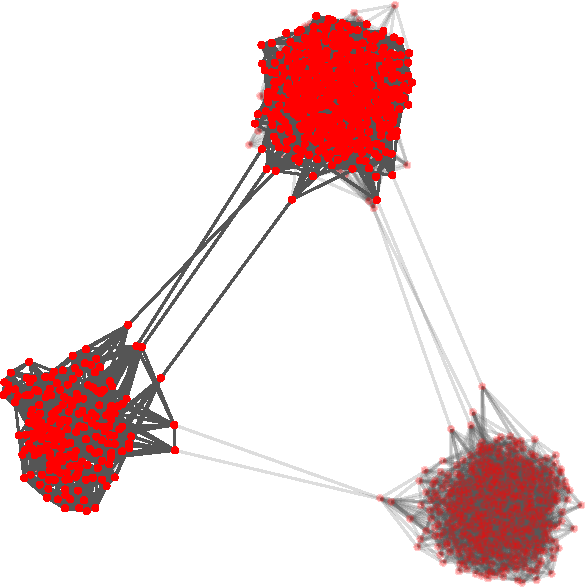
\includegraphics[width=0.3\textwidth]{batchRun__kHalf=6-6-6_maxUpdate=0.02_noize=0_nbrDepth=1/network1000-crop.pdf}
\hskip2cm
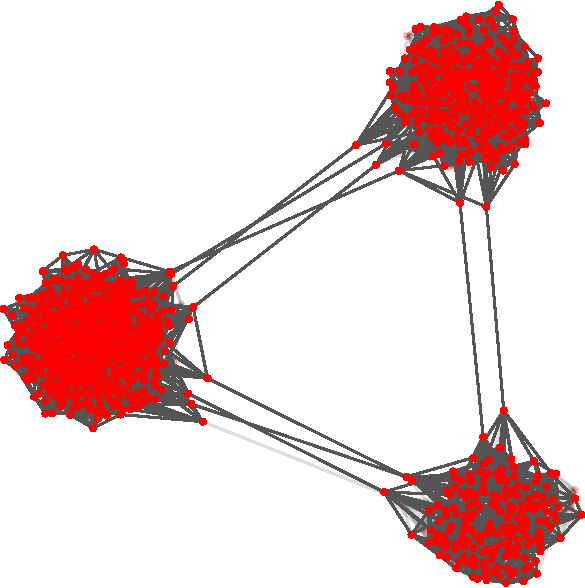
\includegraphics[width=0.3\textwidth]{batchRun__kHalf=6-6-6_maxUpdate=0.02_noize=0_nbrDepth=2/network1000-crop.pdf}

\caption{For this graphs we used a small world network with mean degree 12, a maximal update of 0.02 and 0 noize. In the left series of plots we had a neighbor depth of 1 and in the right series a neighbor depth of 2.}
\label{influencenbrdepth}
\end{figure}

\subsubsection{Influence of the threshold distribution}
\label{sec:influencethresholddistribution}

The figures \ref{infuencethresholdplot} and \ref{inufencethersholdnetwork} show, that the revolution can only cascades without hindrance if the thresholds are distributed stair like as described in \ref{Kuran}. The uniformly distributed threshold we use, equals a stair like distribution with infinitely small steps. In the extreme case in with we set a threshold of 0.2, for 50\% of the agents, the growth of the opposition stops very soon at a low level. the more moderate case of a threshold of 0.4 for half of the agents, the growth of the oppsition isn't prevented, but clearly hindered and slowed down.
On the other hand a threshold distribution that is a favourable for the opposition, like in the example with a threshold of 0.6, the growth of the opposition gets accelerated and the opposition reaches greater percentage of the network.  


\begin{figure}
  \centering
  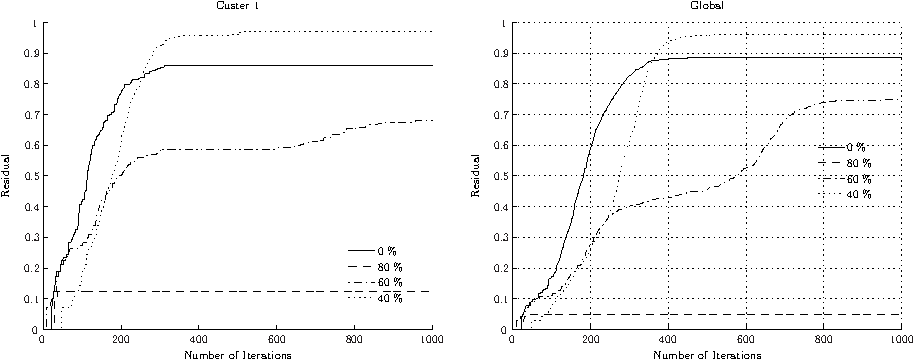
\includegraphics[width= \textwidth]{influenceOffixedthresholds/thresholdinfuence.pdf}
  \caption{The left shows the residual for the cluster in which the riots started, while the right shows the residual over all cluster. Both show the different results for a threshold of 0.0, 0.2, 0.4 and 0.6, for half of the agents. The other half of the agents still have a uniformily distributed threshold.} 
  \label{influencethresholdplot}
\end{figure}





\begin{figure}
\centering
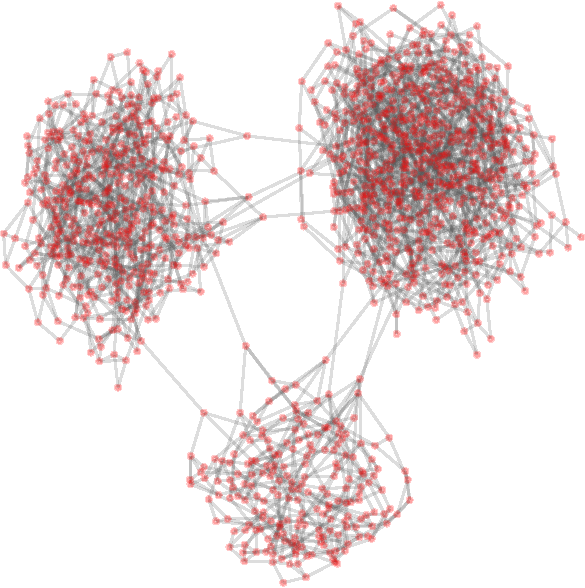
\includegraphics[width=0.25\textwidth]{batchRun__kHalf=2-2-2_maxUpdate=0.08_noize=0_nbrDepth=2/network0-crop.pdf}
\hfill
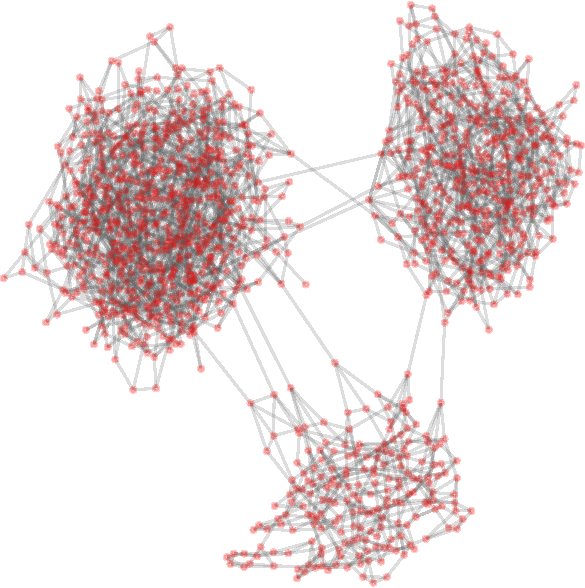
\includegraphics[width=0.25\textwidth]{batchRun__kHalf=2-2-2_maxUpdate=0.08_noize=0_nbrDepth=2_fixedthreshold=0.4/network0-crop.pdf}
\hfill
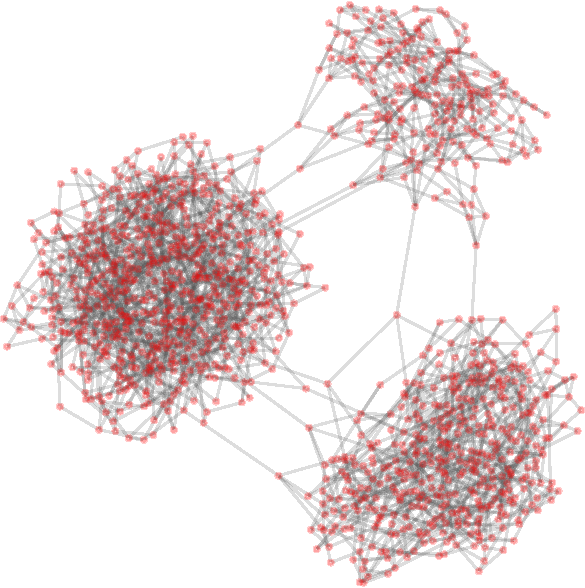
\includegraphics[width=0.25\textwidth]{batchRun__kHalf=2-2-2_maxUpdate=0.08_noize=0_nbrDepth=2_fixedthreshold=0.2/network0-crop.pdf}

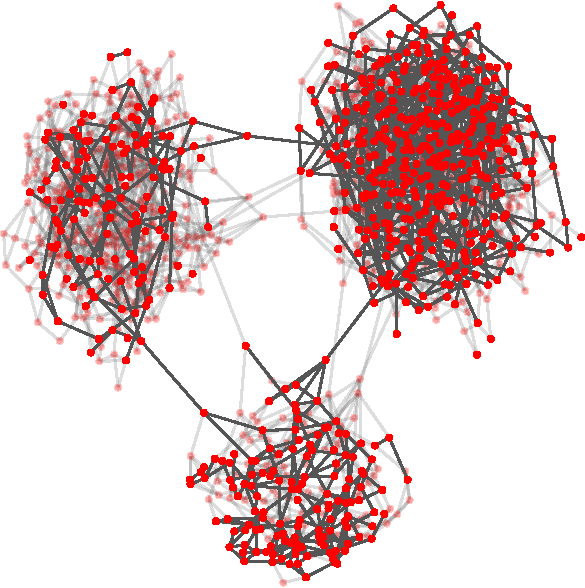
\includegraphics[width=0.25\textwidth]{batchRun__kHalf=2-2-2_maxUpdate=0.08_noize=0_nbrDepth=2/network250-crop.pdf}
\hfill
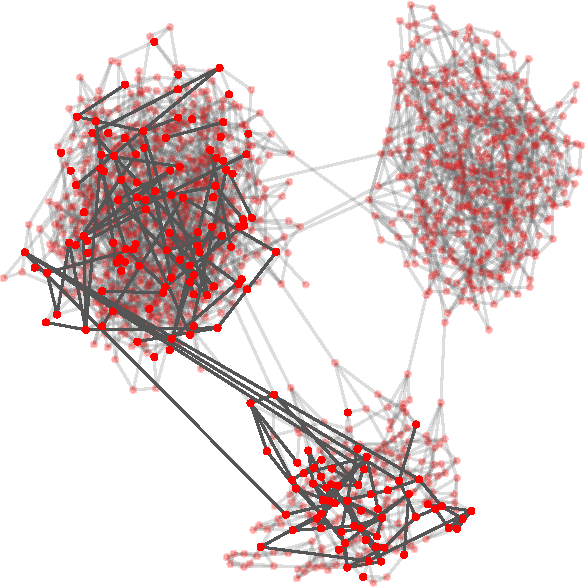
\includegraphics[width=0.25\textwidth]{batchRun__kHalf=2-2-2_maxUpdate=0.08_noize=0_nbrDepth=2_fixedthreshold=0.4/network250-crop.pdf}
\hfill
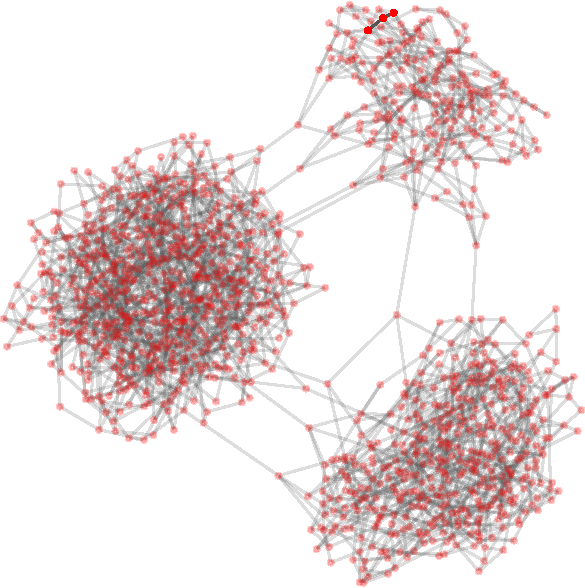
\includegraphics[width=0.25\textwidth]{batchRun__kHalf=2-2-2_maxUpdate=0.08_noize=0_nbrDepth=2_fixedthreshold=0.2/network250-crop.pdf}

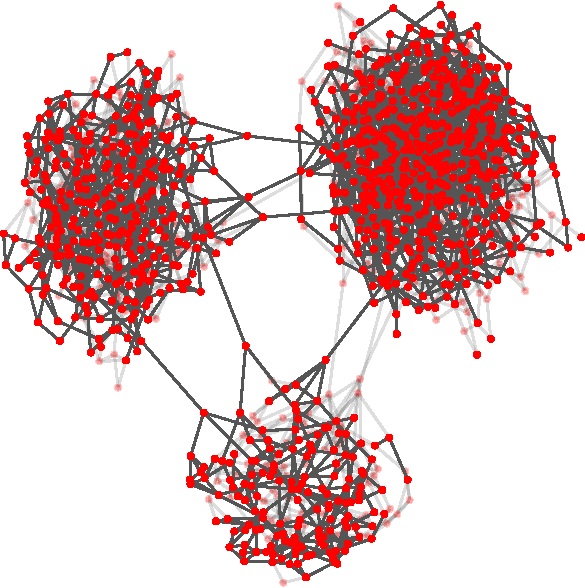
\includegraphics[width=0.25\textwidth]{batchRun__kHalf=2-2-2_maxUpdate=0.08_noize=0_nbrDepth=2/network500-crop.pdf}
\hfill
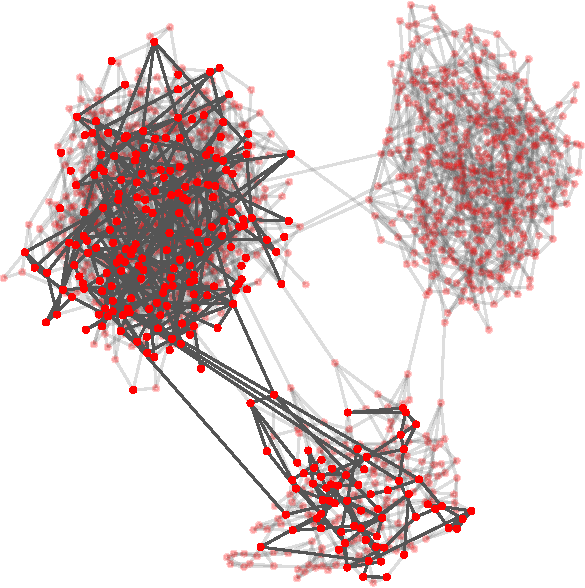
\includegraphics[width=0.25\textwidth]{batchRun__kHalf=2-2-2_maxUpdate=0.08_noize=0_nbrDepth=2_fixedthreshold=0.4/network500-crop.pdf}
\hfill
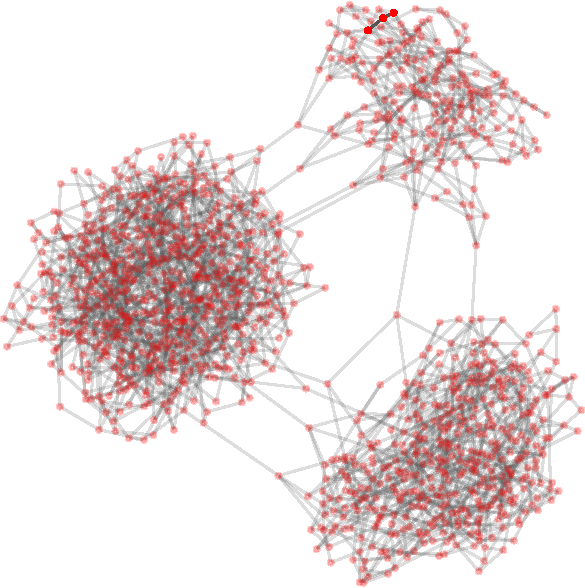
\includegraphics[width=0.25\textwidth]{batchRun__kHalf=2-2-2_maxUpdate=0.08_noize=0_nbrDepth=2_fixedthreshold=0.2/network500-crop.pdf}

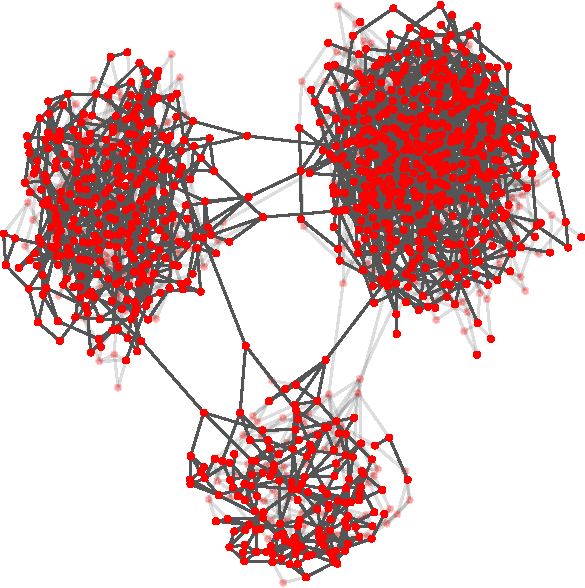
\includegraphics[width=0.25\textwidth]{batchRun__kHalf=2-2-2_maxUpdate=0.08_noize=0_nbrDepth=2/network750-crop.pdf}
\hfill
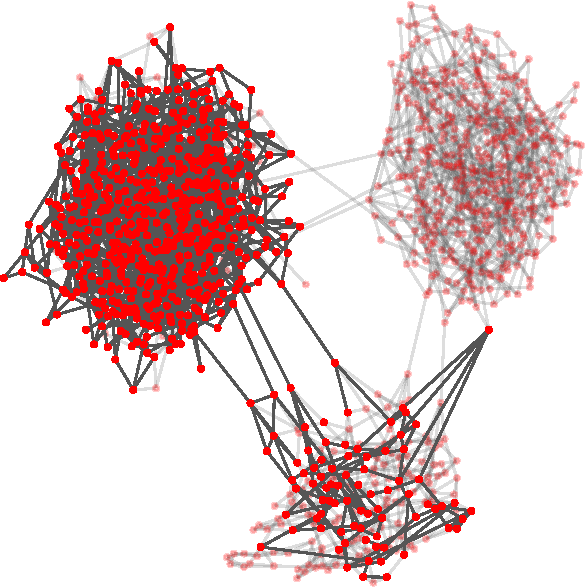
\includegraphics[width=0.25\textwidth]{batchRun__kHalf=2-2-2_maxUpdate=0.08_noize=0_nbrDepth=2_fixedthreshold=0.4/network750-crop.pdf}
\hfill
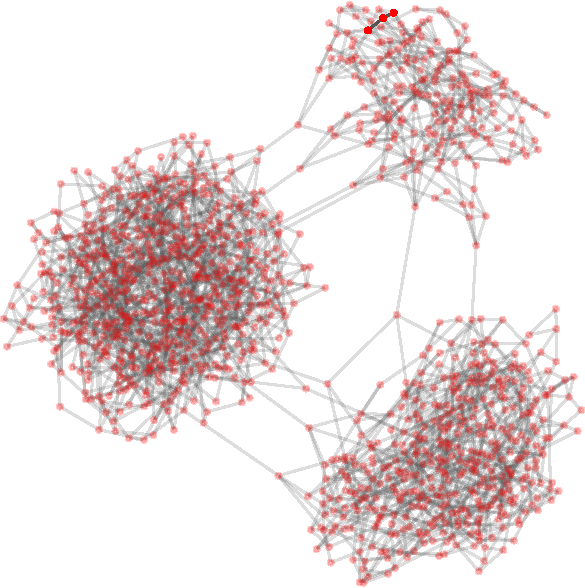
\includegraphics[width=0.25\textwidth]{batchRun__kHalf=2-2-2_maxUpdate=0.08_noize=0_nbrDepth=2_fixedthreshold=0.2/network750-crop.pdf}

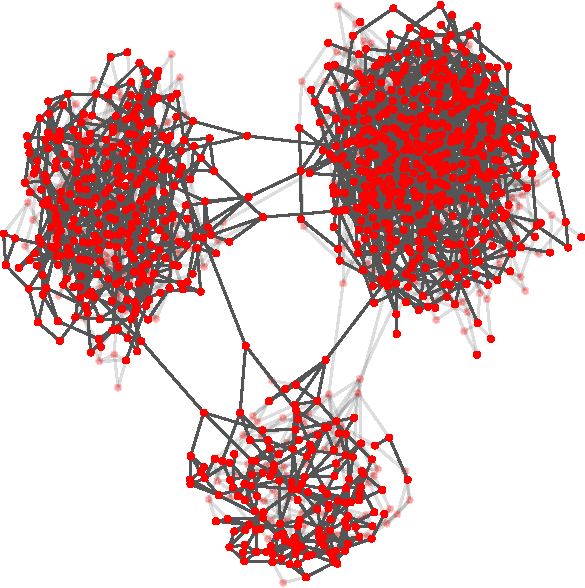
\includegraphics[width=0.25\textwidth]{batchRun__kHalf=2-2-2_maxUpdate=0.08_noize=0_nbrDepth=2/network1000-crop.pdf}
\hfill
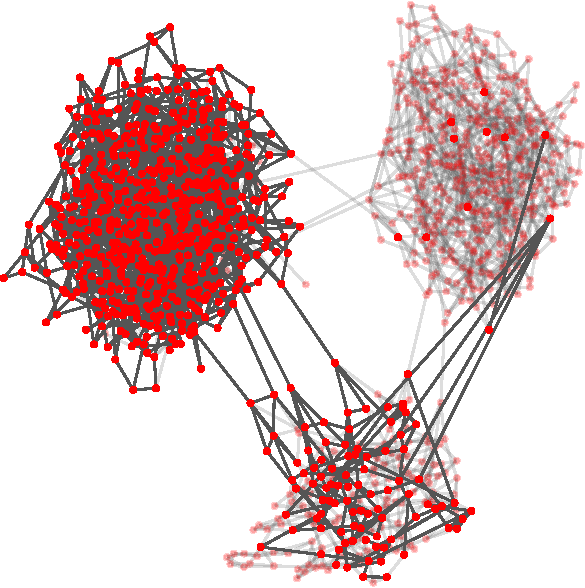
\includegraphics[width=0.25\textwidth]{batchRun__kHalf=2-2-2_maxUpdate=0.08_noize=0_nbrDepth=2_fixedthreshold=0.4/network1000-crop.pdf}
\hfill
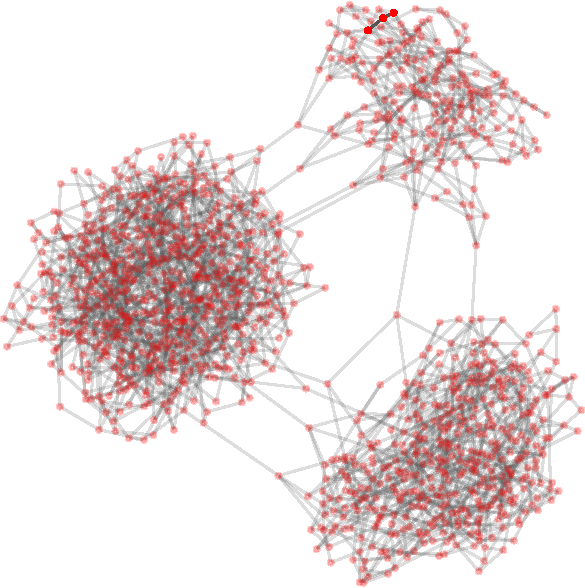
\includegraphics[width=0.25\textwidth]{batchRun__kHalf=2-2-2_maxUpdate=0.08_noize=0_nbrDepth=2_fixedthreshold=0.2/network1000-crop.pdf}

\caption{For this graphs we used a small world network with mean degree 12, a maximal update of 0.08, 0 noize and a neighbour depth of 2. The left graphs are for comparison, while the middle and right graphs are generated with a not uniformly distributed threshold. In the the middle graphs half of the agents have a threshold of 0.4 and in the right graphs one of 0.2. The other half of the agents stays uniformly distributed.}
\label{influencenthresholdnetwork}
\end{figure}

\subsubsection{Influence of the network type}
\label{sec:influencenetworktype}


\begin{figure}
\centering
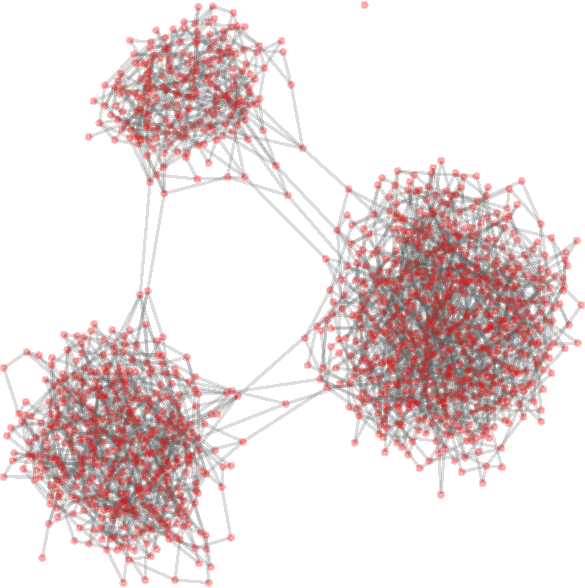
\includegraphics[width=0.3\textwidth]{randomgraphnbrdepth1/network0-crop.pdf}
\hskip2cm
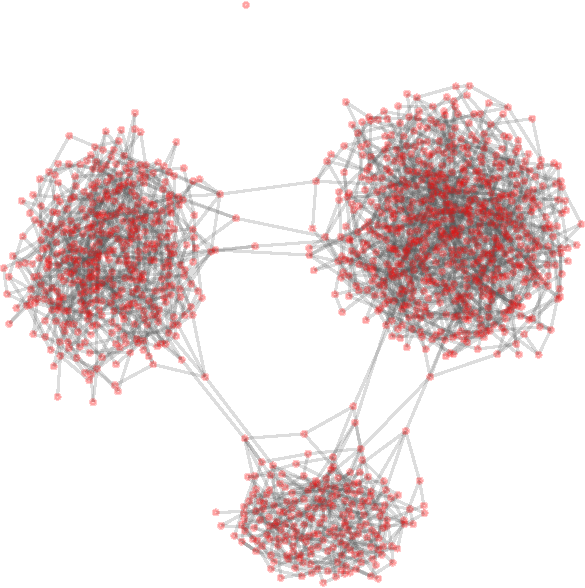
\includegraphics[width=0.3\textwidth]{randomgraphnbrdepth2/network0-crop.pdf}

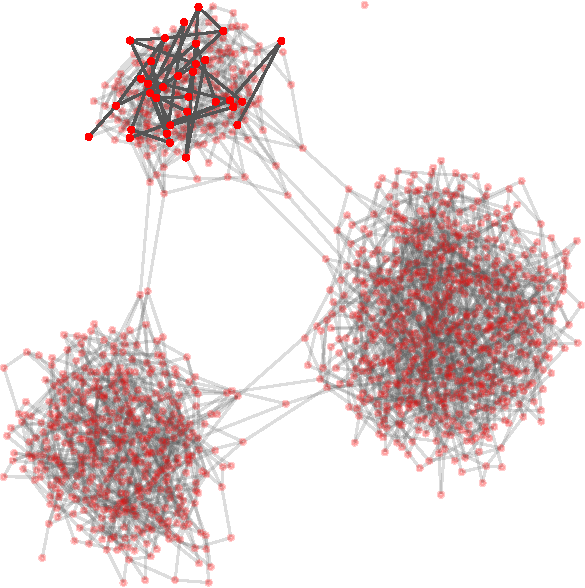
\includegraphics[width=0.3\textwidth]{randomgraphnbrdepth1/network250-crop.pdf}
\hskip2cm
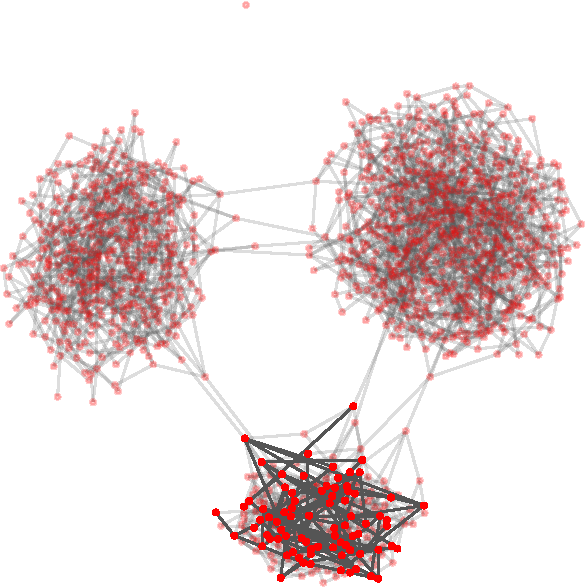
\includegraphics[width=0.3\textwidth]{randomgraphnbrdepth2/network250-crop.pdf}

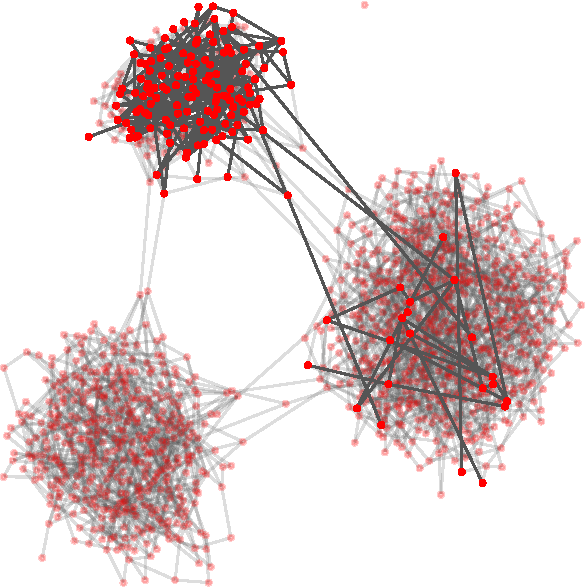
\includegraphics[width=0.3\textwidth]{randomgraphnbrdepth1/network500-crop.pdf}
\hskip2cm
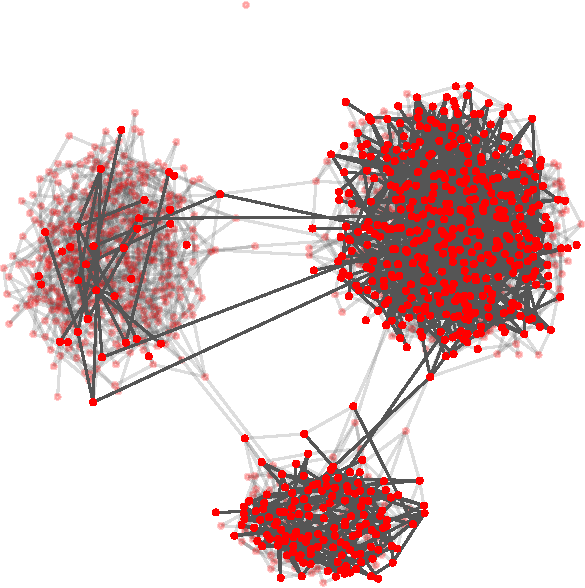
\includegraphics[width=0.3\textwidth]{randomgraphnbrdepth2/network500-crop.pdf}

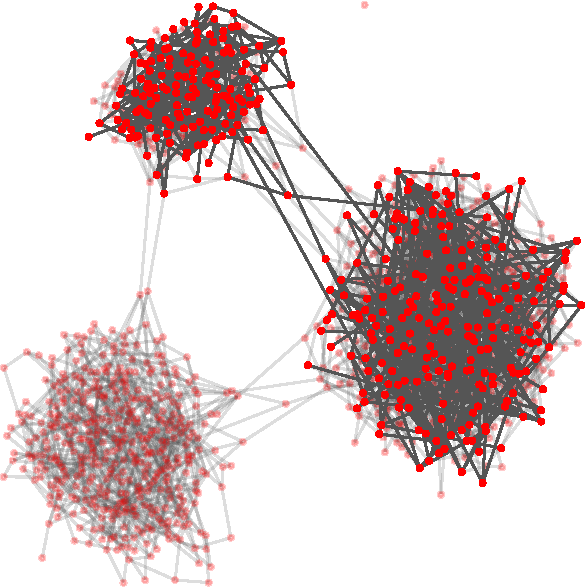
\includegraphics[width=0.3\textwidth]{randomgraphnbrdepth1/network750-crop.pdf}
\hskip2cm
\includegraphics[width=0.3\textwidth]{randomgraphnbrdepth2/network750-crop.pdf}

\includegraphics[width=0.3\textwidth]{randomgraphnbrdepth1/network1000-crop.pdf}
\hskip2cm
\includegraphics[width=0.3\textwidth]{randomgraphnbrdepth2/network1000-crop.pdf}

\caption{The figure above shows the influence of the neighbor depth for the spread of riots in a random network. The total network has a size of 1200.}
\label{influenceNBRdepthRANDOM}
\end{figure}

\subsection{Comparison with a Real Experiment}
\label{sec:comparisontoreal}

So far we were not able to verify the simulated data with real data related to
the Arabian Spring development in northern Africa.  There is not enough time to
research data regarding the Arabian Spring.  However, there is a possibility
for comparison to a similar experiment presented in~\cite{centola2010spread}.
The author tested the effects of network structures on behavioral diffusion.
The study involved randomly assigned participants to join a health community in
the internet.  The behavior of the agents was based on the decision of whether
to join an online health forum or not, based on the action of their
``health-buddies''.  The similarity to the implemented model in
Section~\ref{sec:implementationMatlab} and experiment is that they share the
same mechanism of decision making and both offer only two choices to make.  The
experiment was conducted on two different network structures, \ie, a small
world network according to~\cite{watts98} and a randomly rewired network.  The
difference, however, is that the implemented model does not have a meaningful
time scale, since no parameter were defined based on real data.  Although, the
characteristics of the decision making over time remains similar.

By comparing Figure~\ref{residualNBRdepth} and Figure~2
in~\cite{centola2010spread}, one can see that with a lower number of neighbors
(Figure~2A in~\cite{centola2010spread}) and a smaller population size,
intersection of the two residuals may be possible.  The simulated data for the
plot in Figure~\ref{residualNBRdepth} was conducted with the parameter
\texttt{kHalf} set to six.  This means that each node has~12 neighbors on the
average (for a neighbor depth of one).  There were only six neighbors for the
experiment.  The left plot in Figure~\ref{residualNBRdepth} shows the residuals
for a neighbor depth of one.  These residuals also intersect each other for a
fewer number of neighbors.  Where eventually, the behavior diffuses faster in
the small world networks for the experiment.  The simulation indicates almost
equal residuals for both types of networks at the end of iteration.  This might
be due to too few iterations or other unknown uncertainties.  On the other
hand, if each agent has~12 direct neighbor agents, then there will be a total
of around~144 direct and indirect neighbors for a neighbor depth two.  The
right plot in Figure~\ref{residualNBRdepth} is for a neighbor depth two.
Compared to Figure~2E and~F in~\cite{centola2010spread}, both show steeper
gradients during the first few time steps.  The small world network then
diffuses information faster than the random network for all later times.

There are indeed similarities between the simulated data and the experiment
conducted on a similar model in~\cite{centola2010spread}.  However, the
presented comparison above is in no way a validation of the model.  It only
shows that both have certain characteristics in common which does relate the
implemented model of Section~\ref{sec:implementationMatlab} to a real situation
in some way.  This may be one as in~\cite{centola2010spread} or an Arabian
Spring movement.  However, a valid parameter set must be determined for both
situations.

%%% Local Variables: 
%%% mode: latex
%%% TeX-master: "master"
%%% End:
